% FILE: figures/delta_threshold_k0.tex
% Delta function and threshold in K0

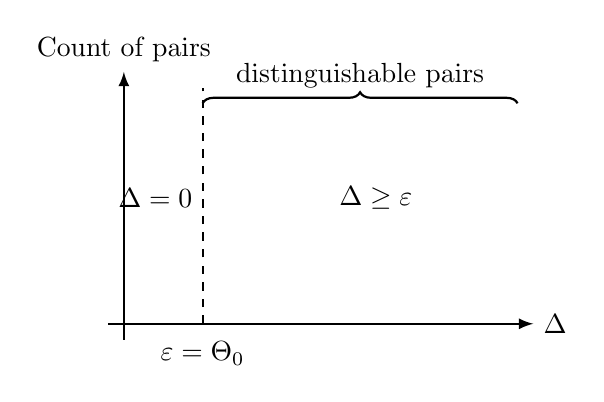
\begin{tikzpicture}[>=latex,thick,scale=1]
  % Axes
  \draw[->] (-0.2,0) -- (5.2,0) node[right] {$\Delta$};
  \draw[->] (0,-0.2) -- (0,3.2) node[above] {Count of pairs};

  % Threshold epsilon line
  \draw[dashed] (1,0) -- (1,3);
  \node[anchor=north] at (1,-0.1) {$\varepsilon=\Theta_0$};

  % Regions
  \node at (0.4,1.6) {$\Delta=0$};
  \node at (3.2,1.6) {$\Delta \geq \varepsilon$};

  \draw[decorate,decoration={brace,amplitude=4pt}] (1,2.8) -- (5,2.8)
    node[midway,anchor=south,yshift=2pt] {distinguishable pairs};
\end{tikzpicture}
